\subsection{Transition into faulty state}
\label{section:transitionToFaultyState}
The moment in time where the typical healthy fingerprint breaks is especially interesting for anomaly detection because it is the earliest fault indication and can be used to avoid total failure. The earlier this happens the more time remains for maintenance or replacement of a damaged part. In the following representation the break is defined as the moment where the fingerprint form significantly changes.
\begin{figure}[H]
    \centering
    \begin{adjustwidth}{-2cm}{-2cm}  % je 2cm links und rechts in den Rand hinein
        \centering
        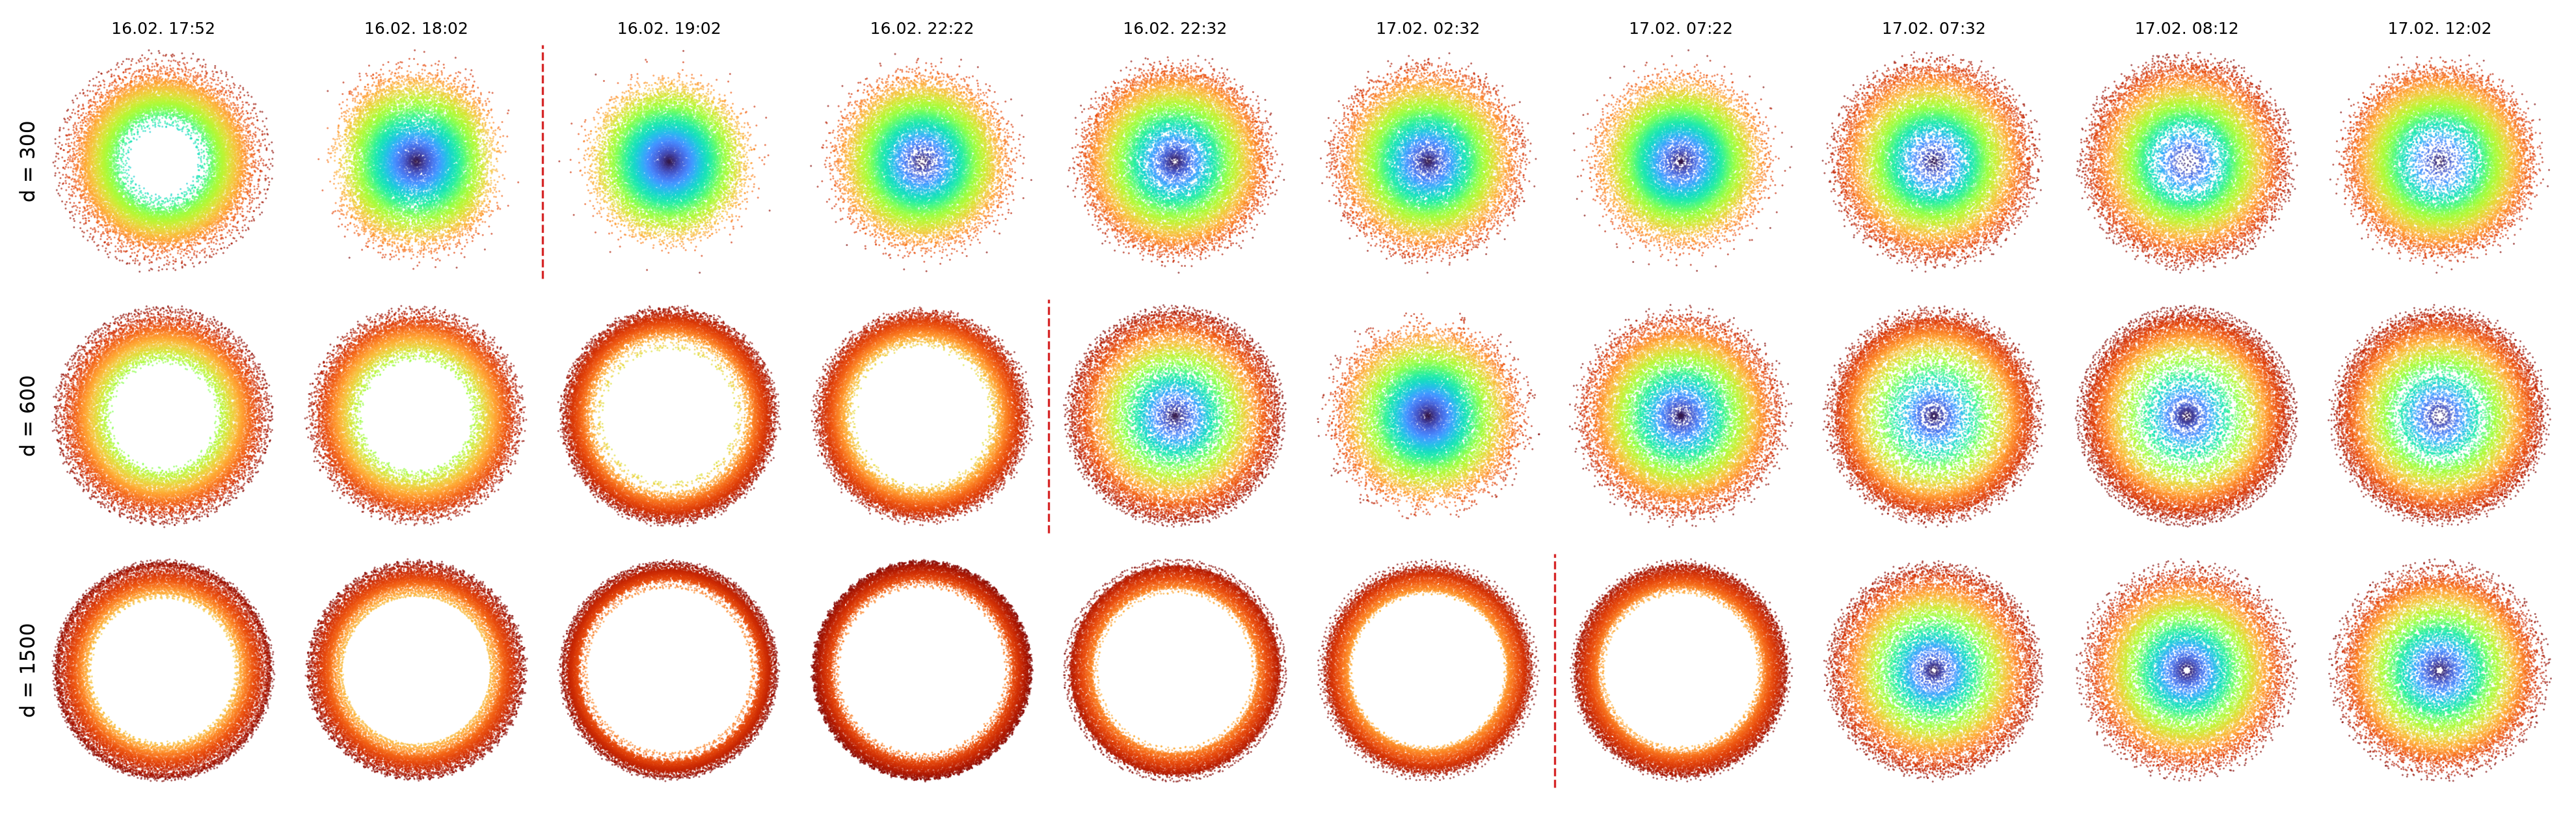
\includegraphics[width=\linewidth]{figures/suddenChanges/break_grid_with_line.png}
    \end{adjustwidth}
    \caption{Run to failure on dataset 2 with different parameter d. The red line indicates a break point.}
    \label{fig:breakPoints}
\end{figure}
As shown in figure \ref{fig:breakPoints}, the dimension parameter $d$ has a significant influence on both the overall form and the time at which a fault is indicated. For smaller dimensions the ring breaks earlier compared to a run with a larger parameter d. Also it is noted that the first plots switch back to the healthy state where the other two stay at a different form long after the fault occurred. A larger $d$ produces a clear and distinct ring that only breaks once the change in the signal is established the choice of d is therefore crucial for stable fault indication. 